\section{V2}
\subsection{Mechanismen der epigenetischen Modifikation}
\begin{description}
    \item[DNA-Methylierung] an CpG-Inseln (hauptsächlich dort) durch DNA-Methyltransferase kann Transkription blockieren
    \item[Histon-Methylierung] (Chromatin remodeling) kann sowohl positiv als auch negativ mit Transkription korrelieren (je nach betroffenen Aminosäuren)
    \item[Histon-Acetylierung] (Chromatin remodeling) kann DNA zugänglicher machen und damit Transkription (auch Translation) beeinflussen
\end{description}
\textbf{Histonmodifikationen und DNA-Methylierung sind vererbbar}

\subsection{Mechanismen der DNA Reparatur}
Mechanismen der DNA-Reparatur sind Basenexzision, Nukleotidexzision, Reparatur von Doppelstrangbrüchen und - als ``Notausstieg'' - der programmierte Zelltod, die Apoptose.

\subsubsection{Basenexcisionsreparatur}
\begin{enumerate}
    \item Glycosylase entfernt defekte Base
    \item Endunuclease entfernt die fehlerhafte Stelle mit umliegenden Nucleotiden und fügt Doppelstrangbruch ein
    \item Polymerase und Ligase füllen die Lücke
\end{enumerate}

\subsubsection{Reparatur von Doppelstrangbrüchen}
p53, der ``Wächter des Genoms'', repariert oder löst Aptoptose aus. Serin-Proteinkinasen aktivieren bei der Registrierung eines Doppelstrangbruches p53, indem dessen Repressor, MDM2, deaktiviert wird. Bei vielen Krebserkrankungen ist p53 nicht funktionsfähig.

\subsection{Typische Mutationen}
Bei der Synthese von DNA-Kopien können Fehler auftreten. Diese Fehler sind zum Teil durchaus sinnvoll, so wird Evolution ermöglicht. Sobald DNA in der Keimbahn mutiert, kann sie als genetische Variante, \textbf{SNP} (single nucleotide polymorphism), vererbt werden.

Ein möglicher Zustand an einem Gen-Locus (= -Ort) wird als \textbf{Allel} bezeichnet. Ein Nachkomme zweier diploider Organismen erbt normalerweise je ein Chromosom der Mutter und eines des Vaters. Damit erhält er je zwei Allele jedes Gens (außer bei Genen, die auf den Geschlechtschromosomen liegen (chrX, chrY; gonsomale Gene)). Die Kombination der beiden Allele des mütterlichen und väterlichen Genlocus heißt \textbf{Genotyp}.

\begin{itemize}
    \item Häufige SNPs
    \item Seltene SNPs
    \item Chromosomenmutationen
    \item Repeats
    \begin{description}
        \item[Megasatelliten] mehrere kbp, Blocks bis 100e kbp
        \item[Satelliten] 5-171 bp, Blocks 100 kbp - Mbp
        \item[Minisatelliten] 6-64 bp, Blocks 0.1 kbp - 20 kbp
        \item[Microsatelliten] 1-4 bp, Blocks bis 150 bp
    \end{description}
    \item Transposons
\end{itemize}

\subsubsection{SNPs (Single Nucleotide Polymorphisms)}
\begin{itemize}
    \item Basenunterschied
    \item Mensch: ca. 3 Mrd Basenpaare
    \item ca. 3 Mio. häufige Basenunterschiede zwischen Individuen
    \item ca. 150 Mio. seltene Basenunterschiede zwischen Individuen
    \item ca. 99.9\% Sequentidentität zwischen Individuen
\end{itemize}

\subsubsection{Chromosomenmutationen}
\textbf{Intrachromosomal}
    \begin{itemize}
        \item Inversion
        \item Duplikation
        \item Deletion
    \end{itemize}
\textbf{Interchromosomal}
    \begin{itemize}
        \item Insertion
        \item Translokation
    \end{itemize}

\subsubsection{CNV (Copy Number Variation)}
\begin{itemize}
    \item Ein DNA-Segment mit mindestens 1 kb, das in variabler Zahl relativ zu einem Referenzgenom vorkommt
    \item Indels und Duplikationen sind CNVs
    \item CNP (Copy Number Polymorphisms)-MAF $>$ 1\%
\end{itemize}

\subsection{PCR (Polymerase-Kettenreaktion)}
Mit speziell designten DNA-Primern wird die Sequenz, die von diesen Primern flankiert wird, von einer thermostabilen DNA-Polymerase amplifiziert. Die verschiedenen Schritte der Kettenreaktion werden, wie im Bild unten zu sehen, mit Hilfe der Temperatur gesteuert.
Um genügend Material für Messungen zu erhalten, wird häufig PCR eingesetzt.

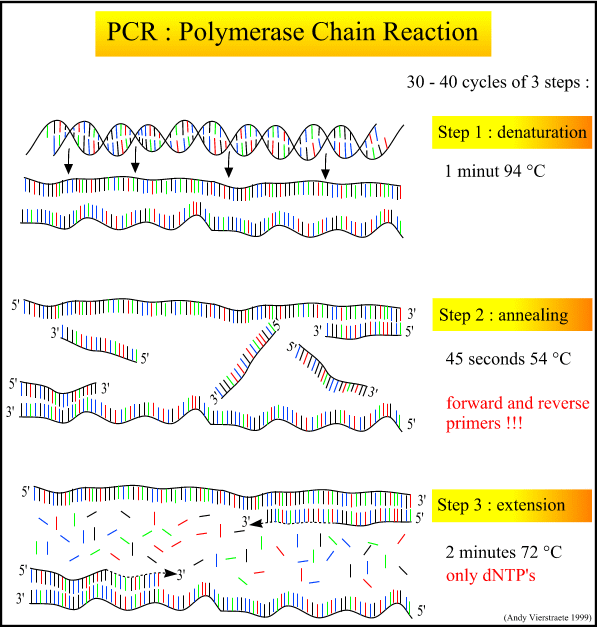
\includegraphics[width=0.5\textwidth]{lectures/V2/pix/pcr1.png}
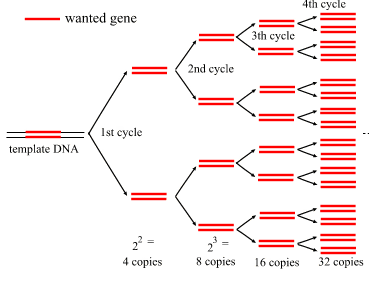
\includegraphics[width=0.5\textwidth]{lectures/V2/pix/pcr2.png}

\subsection{Sanger Sequenzierung}
Bei der sogenannten ``Kettenabbruch''-Methode nach Sanger wird ausgehend von einem Primer in Einzelstränge aufgetrennte DNA mittels Polymerase vervollständigt. Für jede Base $\{A, T, G, C\}$ wird jeweils ein eigener Ansatz hergestellt, in dem zusätzlich zu den vier normalen dNTPs \textbf{d}dNTPs für je eine der Basen beigmischt werden. ddNTPs fehlt die 3'-Hydroxygruppe, außerdem können sie fluoreszenzmarkiert (oder radioaktiv markiert) werden. Wird nun während des Sequenzierungsprozesses ein ddNTP in den wachsenden DNA-Strang eingebaut, bricht die Polymerase an dieser Stelle aufgrund der besonderen Eigenschaften (fehlendes 3'-OH) der ddNTPs ab. Zufällig kann nun an jeder Stelle ein ddNTP eingebaut werden, was zu je einer spezifischen Länge des resultierenden Fragments führt.

Die entstandenen Fragmente können nun mittels Gelelektrophorese aufgetrennt werden, um jeweils die Abbruchstellen bei der Zugabe einer bestimmten ddNTP-Art (A, T, G, C) festzustellen.
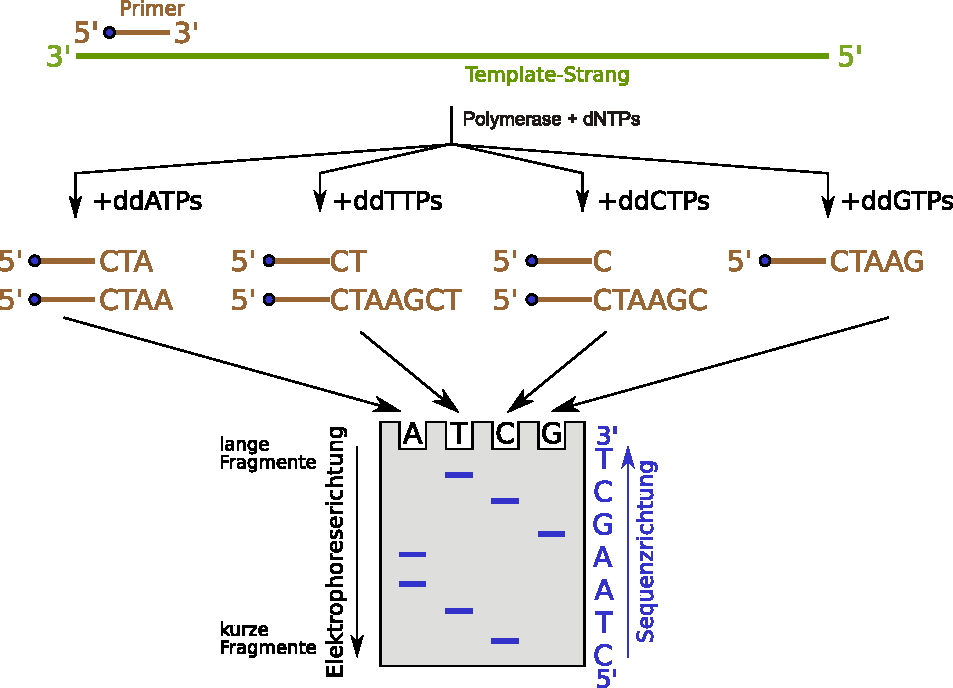
\includegraphics[width=0.5\textwidth]{lectures/V2/pix/Didesoxy-Methode.pdf}

\subsection{TaqMan}
Die TaqMan-SNP-Genotypisierungstechnik nutzt die 5'-Nuklease-Aktivität der Taq-Polymerase, um ein Fluoreszenzsignal während der PCR zu emittieren. Für jedes SNP werden zwei TaqMan-Sonden beigemischt, deren Sequenz sich nur an der SNP-Stelle unterscheidet. Eine der Sonden ist dabei komplementär zum Wildtyp-Allel und die andere zum Varianten-Allel. Genutzt wird hier die FRET-Technik mit einem 5'-Reporter-Dye und einem 3'-Quencher-Dye, die je kovalent and die Sonden gebunden sind. Das Quencher-Dye verhindert, bei unmittelbrer Nähe zum Reporter, das Leuchten desselben. Sind die Sonden intakt, ist die Fluoreszenz unterdrückt, da sich die Quencher-Dyes in der Nähe der Reporter-Dyes befinden. Im PCR-Annealing-Schritt hybridisieren die TaqMan-Proben mit der SNP-Stelle. Während der PCR-Elongation werden Reporter- und Quencher-Dyes durch die 5'-Nuklease-Aktivität der Taq-Polymerase freigesetzt. Dies führt zu einer charakteristischen Fluoreszenz-Aktivität der Reporter-Dyes. Die Taq-Polymerase wirkt nur bei perfekter Hybridisierung der Probe als Exonuklease, da die Probe mit einem Mismatch von der Exonuklease nicht erkannt wird.

Am Ende der PCR-Reaktion wird das Fluoreszenz-Signal gemessen. Das Verhältnis der Signale lässt nun Rückschlüsse auf den Gentyp zu.

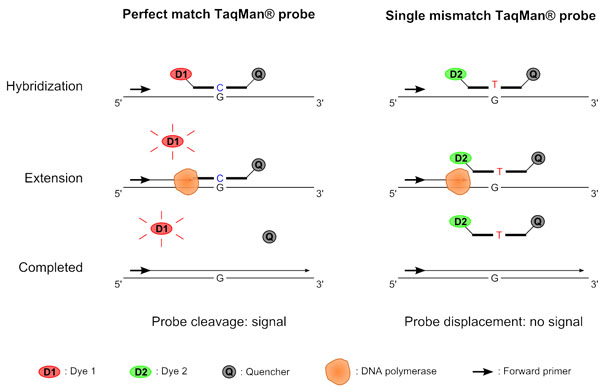
\includegraphics[width=0.75\textwidth]{lectures/V2/pix/snpcalling1.png}

\subsection{SNP-Microarrays}

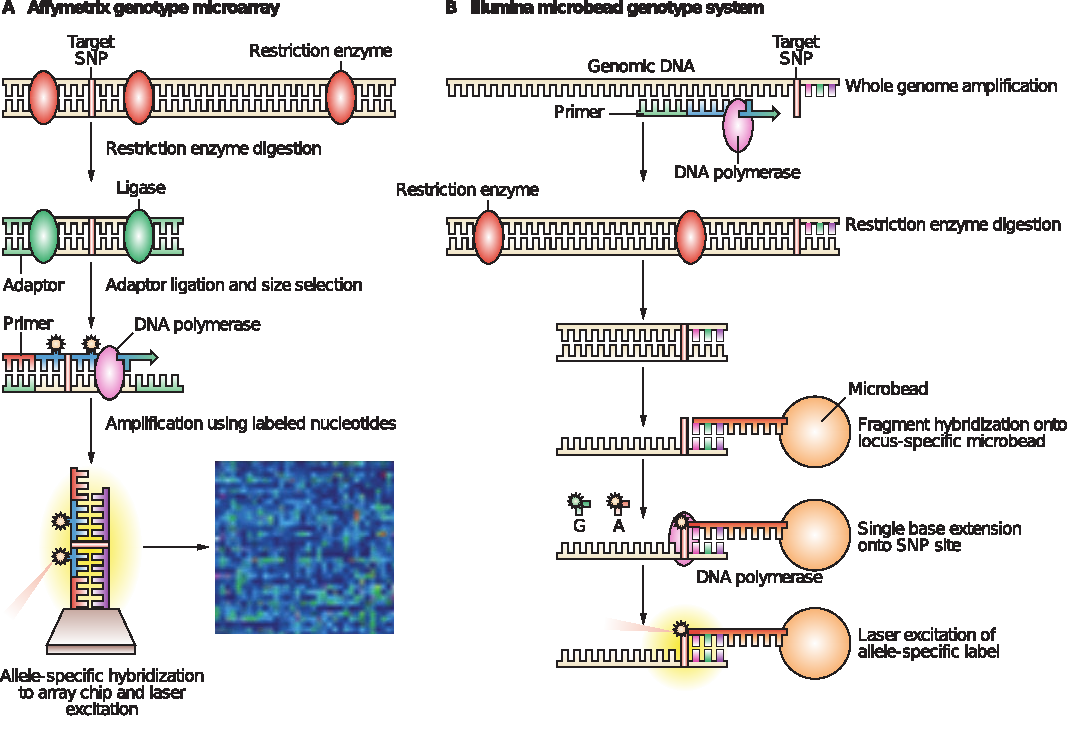
\includegraphics[width=1\textwidth]{lectures/V2/pix/snp_arrays.pdf}

Zwei Hochdurchsatz-SNP-Genotypisierungsplattformen für genomweite Assoziationsstudien.

\begin{description}
    \item[(A)] SNP-Genotypisierung mittels Affymetrix Microarrays. Genomische DNA wird durch Restriktionsenzyme verdaut. 
        Um universelle Primer-Schnittstellen für die PCR zu erhalten, werden Adapter an die Fragmentenden ligiert. 
        Fragmente der Größe 250 – 1000 bp werden amplifiziert, fluoreszenzmarkiert und an das Array hybridisiert. 
        Diese Arrays werden gescannt und die SNP-Genotypen werden, nach der Laser-Detektion, mit ``spezieller Software'' erkannt.
    \item[(B)] SNP-Genotypisierung mit Illumina-Bead-Arrays. Genomische DNA wird genomweit amplifiziert und die amplifizierte DNA dann durch Restiktionsenzyme verdaut. 
        Die Fragmente werden nun mit SNP-spezifischen Bead-Chips hybridisiert, die je zwei Sonden tragen, die es erlauben, beide SNP-Allele simultan zu genotypisieren. 
        Sie binden an die DNA-Muster an der Base direkt vor dem SNP.
        Die gebundene DNA wird nun, abhängig vom SNP-Genotyp, um eine einzige gelabelte Base verlängert.
        Die verlängerten Proben werden nun angefärbt, um das Signal zu verstärken und um die Detektion der eingebauten Base mittels Laser-Anregung zu erlauben. 
        Auch hier werden die Genotypen mit einem Array-Reader und ``spezieller Software'' detektiert.
\end{description}

\subsection{Aufgaben zur Übung 2}
\subsubsection{Aufgabe 1}
\textbf{a.)}\\
Als Crossing-over\footnote{\url{https://de.wikipedia.org/wiki/Crossing-over}} wird in der Genetik eine kreuzweise Überlagerung zweier Chromatiden mit nachfolgendem, gegenseitigem Austausch von Abschnitten bezeichnet, wie er zwischen väterlichen und mütterlichen homologen Chromosomen bei einer Meiose auftreten kann.
\\\\

\textbf{b.)} A und B sind rekombiniert zu C,D,E

\textbf{c.)} A, D,E sind rekombiniert mit B,C

\textbf{zu b.)}\hspace*{65mm}\textbf{zu c.)}\\\\
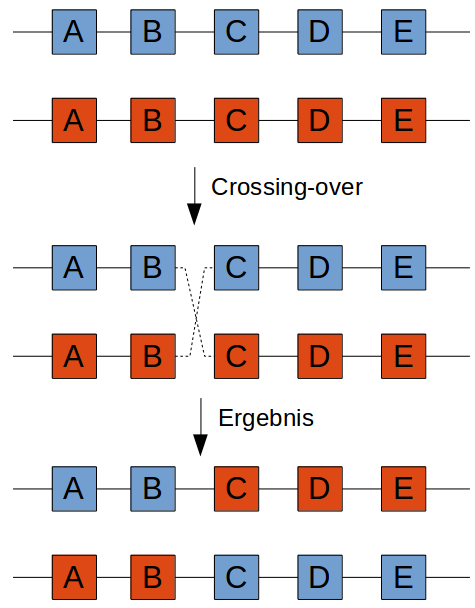
\includegraphics[width=0.5\textwidth]{lectures/V2/pix/crossing_over_b.png}
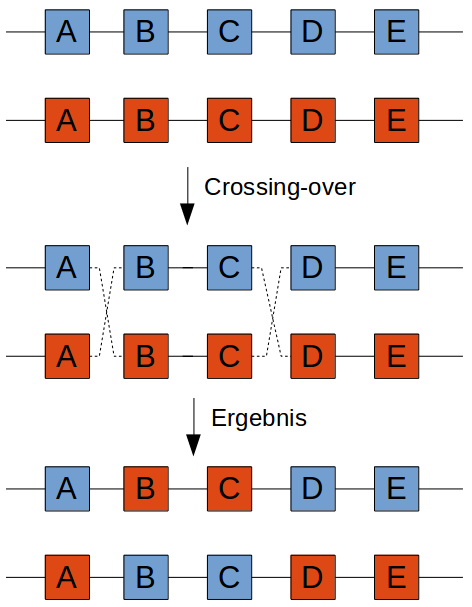
\includegraphics[width=0.5\textwidth]{lectures/V2/pix/crossing_over_c.png}

\subsubsection{Aufgabe 2}
Gen: ABO\footnote{\url{http://www.snpedia.com/index.php/ABO}}
rs8176719\footnote{\url{http://www.snpedia.com/index.php/rs8176747}}:
\begin{itemize}
	\item (-;-): likely to be of blood type O
	\item (-;G): most likely to be of blood type A or B
	\item (G;G): most likely to be of blood type A, B or AB 
\end{itemize}

rs8176747\footnote{\url{http://www.snpedia.com/index.php/rs8176747}}:
\begin{itemize}
	\item G führt zu Blutgruppe A, C zu Blutgruppe B
\end{itemize}

rs8176750\footnote{\url{http://www.snpedia.com/index.php/rs8176750}}: definiert Untergruppe von A
\begin{itemize}
	\item (-;C): A1
	\item (-;-): A2
\end{itemize}

Kombinationsmöglichkeiten:
\begin{itemize}
	\item praktisch durch Allele vorgegeben: $3 \cdot 2 \cdot 2 = 12$\footnote{\url{https://sites.google.com/site/abobloodgroup/14.aboalleles\%28oalleles\%29}}
	\item theoretisch: $5^3=125$
	\item \underline{Musterlösung:} 3 SNPs auf einem Allel $\rightarrow$ 8 Kombinationen; 2 Allele: 36 Möglichkeiten
\end{itemize}

A und B kodominant, Faktor 0 rezessiv

\subsubsection{Aufgabe 3}

\textbf{a.)}

\textbf{b.)}

\textbf{c.)}

\subsubsection{Aufgabe 4}

\textbf{a.)}\\
\underline{rezessiv:}\footnote{\url{https://de.wikipedia.org/wiki/Rezessiv}} bedeutet in der Genetik „zurücktretend“ oder auch „nicht in Erscheinung tretend“

\underline{dominant:}\footnote{\url{https://de.wikipedia.org/wiki/Dominanz_(Genetik)}} ein dominantes Allel setzt sich in der Merkmalsausprägung gegenüber einem rezessiven Allel durch

\underline{Penetranz:}\footnote{\url{https://de.wikipedia.org/wiki/Penetranz_(Genetik)}} prozentuale Wahrscheinlichkeit, mit der ein bestimmter Genotyp zur Ausbildung des zugehörigen Phänotyps führt
\\\\
\textbf{b.)}\\
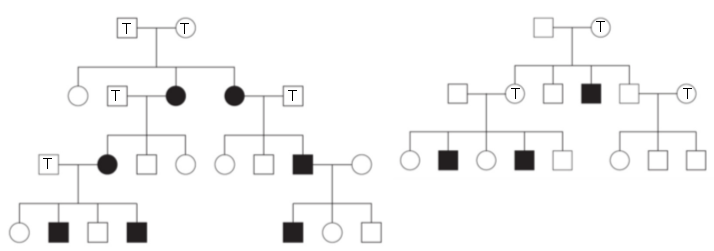
\includegraphics[width=1\textwidth]{lectures/V2/pix/stammbaeume1.png}
\newpage
\underline{aus Musterlösung:}\\
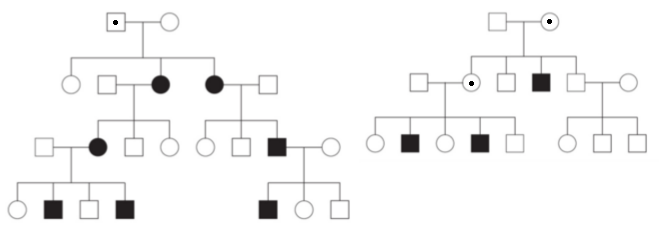
\includegraphics[width=1\textwidth]{lectures/V2/pix/standard_solution.png}
\\\\
\textbf{c.)}\\
\underline{links:} autosomal rezessiv, \underline{aus Musterlösung:} autosomal dominat mit reduzierter Penetranz, weil:
\begin{itemize}
	\item beide Geschlechter betroffen
	\item in jeder Generation
	\item etwa die Hälfte der Kinder betroffen
\end{itemize}

\underline{rechts:} genosomal rezessiv, auf einem X-Chromosom der Mutter\\
